\documentclass{article}
\usepackage{graphicx}
\usepackage{amsmath, stackrel, amssymb}
\usepackage{mathtools}
\usepackage{scrextend}
\usepackage{xcolor}
\usepackage[a4paper, top=15mm, bottom=20mm]{geometry}
\title{Proyecto de Simulación	
    \\
    \large Predicción de resultados en la MLB}

\author{Alejandro Álvarez Lamazares - C311
\\
        Marian S. Álvarez Suri - C312
        \\
        Carlos A. Bresó Sotto - C312}
\date{}

\begin{document}
    \maketitle
    \large

    \section{Introducción}

        \subsection{Breve descripción del proyecto}
            Este proyecto tiene como objetivo utilizar una simulación de eventos discretos y el análisis de una tabla de estadísticas de la Major League Baseball (MLB) para predecir los resultados de un intervalo de fechas. Se busca anticipar el clasificador final de la tabla de posiciones basándose exclusivamente en los datos disponibles hasta el momento definido por el usuario.

        \subsection{Objetivos y metas}
            El propósito de este proyecto es aproximarse lo más posible al resultado factual de la temporada de la MLB. Se evaluará la precisión de las simulaciones utilizando los datos reales del problema como base.

        \subsection{Variables que describen el problema}
            Se realizará una simulación de un rango determinado de una temporada de la MLB, utilizando los resultados previamente. Se incorporarán variables adicionales, como las posibles lesiones de jugadores, que podrían influir en el desenlace de cada partido.

    \section{Detalles de implementación}

        El código comienza importando las bibliotecas necesarias: pandas para el manejo de datos, random para la generación de números aleatorios y numpy para las operaciones matemáticas.

        A continuación, se explicará el código por funciones:

        \begin{itemize}
            \item[\checkmark] \textbf{\textcolor{blue}{load\_data(filename)}}: Se utiliza para cargar los datos necesarios para la simulación. La función toma un nombre de archivo como argumento y utiliza la biblioteca pandas para cargar los datos en un DataFrame.
            \item[\checkmark] \textbf{\textcolor{blue}{get\_history(team1, team2, results)}}: devuelve el número de partidos jugados y ganados entre dos equipos.
            \item[\checkmark] \textbf{\textcolor{blue}{simulate\_injured\_players(p=0.5)}}: simula si hay jugadores lesionados en un equipo, utilizando una distribución binomial con $p = 0.5$, donde $p$ es la probabilidad de éxito.
            \item[\checkmark] \textbf{\textcolor{blue}{simulate\_game(team1, team2, results, game\_simulations)}}: simula un partido entre dos equipos basándose en los resultados históricos y en la posibilidad de que haya jugadores lesionados. Para esto, se calcula una tasa llamada "win\_rate", que se utiliza en una simulación de Monte Carlo para estimar el ganador del partido.
            \item[\checkmark] \textbf{\textcolor{blue}{simulate\_season(statistics, game\_simulations, count)}}: simula una temporada completa, haciendo que cada equipo juegue contra todos los demás. Por cada par de equipos, se simula el juego y se guardan los resultados.
            \item[\checkmark] \textbf{\textcolor{blue}{create\_results\_table(total\_wins)}}: convierte los resultados de la simulación en un DataFrame de pandas y lo ordena por el número total de victorias.
            \item[\checkmark] \textbf{\textcolor{blue}{create\_histogram(statistics, total\_spots, n)}}: Genera un histograma que representa la frecuencia de cada posición (spot) para los primeros $n$ equipos seleccionados.
            \item[\checkmark] \textbf{\textcolor{blue}{get\_sim\_results(epsilon, game\_simulations=100, show\_table=False, show\_histogram=True, num\_teams=5)}}: Realiza simulaciones de juegos con varios equipos y recopila los resultados. El parámetro 'epsilon' controla qué tanto tiempo estará ejecutándose la simulación según la desviación estándar de la distribución normal.
            \item[\checkmark] \textbf{\textcolor{blue}{get\_real\_results()}}: Obtiene los resultados reales de los juegos en un rango de tiempo determinado a partir de las estadísticas de la MLB.
            \item[\checkmark] \textbf{\textcolor{blue}{position\_distances(df\_real, df\_simulated)}}: Calcula la distancia promedio entre las posiciones reales y simuladas de cada equipo a lo largo de varias ejecuciones. La distancia se calcula como la diferencia absoluta entre las posiciones reales y simuladas.
            \item[\checkmark] \textbf{\textcolor{blue}{exact\_positions(df\_real, df\_simulated)}}: Calcula el número de equipos que tienen la misma posición en los resultados reales y simulados creando una nueva columna que es Verdadera cuando las posiciones son las mismas y Falsa en caso contrario.
            \item[\checkmark] \textbf{\textcolor{blue}{top\_n(df\_real, df\_simulated, n)}}: Cuenta cuántos de los primeros $n$ equipos coinciden en sus posiciones en los resultados reales y simulados. 
            \item[\checkmark] \textbf{\textcolor{blue}{spearman\_correlation(df\_real, df\_simulated)}}: Calcula la correlación de Spearman entre las posiciones reales y simuladas de cada equipo.
            \item[\checkmark] \textbf{\textcolor{blue}{print\_results(num\_simulations, game\_simulations)}}: Ejecuta todo el proceso varias veces y devuelve la distancia media entre las posiciones reales y simuladas de los equipos.
            \item[\checkmark] \textbf{\textcolor{blue}{run\_simulation(epsilon, game\_simulations, show\_table=False)}}: Ejecuta una simulación de juegos y compara los resultados de la simulación con los resultados reales. Se obtienen los resultados reales con \textit{get\_real\_results()}. Luego, obtiene los resultados simulados llamando a \textit{get\_sim\_results(epsilon, game\_simulations, show\_table, True)}. Después de obtener los resultados reales y simulados, calcula la distancia de las posiciones entre ellos, el número de posiciones exactas, el número de equipos en las primeras $n$ posiciones que coinciden en los resultados reales y simulados, y la correlación de Spearman entre las posiciones reales y simuladas. Finalmente, devuelve una lista con estos cuatro resultados.
        \end{itemize}

    \section{Resultados y experimentos}
        La simulación realizada ha mostrado una notable coincidencia con los resultados finales de la temporada observada. A continuación, se presenta una representación gráfica que ilustra la comparación entre los datos reales y los obtenidos a través de la simulación.

        \begin{figure}[h!]
            \begin{center}	
                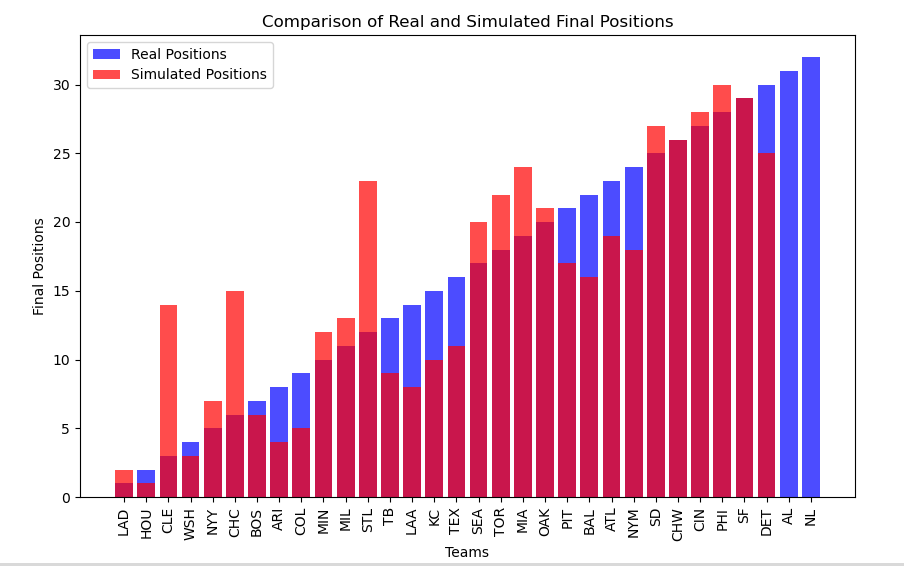
\includegraphics[width=1.0\linewidth]{bar_chart.png}
            \end{center}
        \end{figure}

        \subsection{Hallazgos de la simulación}
            Los valores obtenidos mediante la simulación evidencian una notable significación de los resultados previos en la tabla final de posiciones, así como de los enfrentamientos particulares entre dos equipos. Sin embargo, los datos sugieren que la relación no es perfecta, puesto que existen desviaciones considerables en las posiciones finales de algunos de los equipos que tuvieron un desempeño particular en el rango de tiempo usado para extraer las estadísticas.
        \subsection{Interpretación de los resultados}
            Los resultados obtenidos sugieren que la simulación es una herramienta eficaz para predecir los resultados de la MLB, siempre y cuando se disponga de datos suficientes y relevantes para alimentar el modelo. La precisión de las predicciones puede variar en función de la calidad y cantidad de los datos utilizados, así como de la complejidad del modelo empleado. En este caso, la simulación ha demostrado ser capaz de predecir con un buen grado de precisión la tabla de posiciones de la MLB.
        \subsection{Hipótesis extraídas de los resultados}
            Basándose en los hallazgos obtenidos, se puede formular la hipótesis de que, mediante el uso de simulaciones, es factible predecir el resultado final de la tabla de posiciones de una temporada de la Major League Baseball. Esto subraya la utilidad de las simulaciones como herramientas predictivas en el ámbito deportivo, especialmente cuando se dispone de datos relevantes.

        \subsection{Experimentos realizados para validar las hipótesis}
            Se realizaron múltiples ejecuciones de la simulación con el objetivo de confirmar que los resultados obtenidos no sean el producto de circunstancias fortuitas o aleatorias, sino que reflejen una tendencia consistente y válida. Este enfoque metodológico permite establecer una mayor confianza en la precisión y fiabilidad de los hallazgos, al minimizar el riesgo de atribuir el éxito de la predicción a factores externos o a la casualidad.

            \textbf{Métricas empleadas:}
            Para validar los resultados empleamos varias métricas que explicaremos a continuación:

            \begin{itemize}
                \item \textbf{Distancia entre posiciones}: Indica la diferencia entre la posición real y la simulada de un equipo. Permite obtener una aproximación general de qué tan cerca están los resultados simulados de los reales. Un elemento negativo a tener en cuenta es que una tabla donde hayan solo dos posiciones intercambiadas puede llegar a ser mucho peor que una donde todas las posiciones tengan un error absoluto de 1.
                \item \textbf{Posiciones exactas}: Muestra cuántas veces la simulación acertó la posición exacta de un equipo. Una de las desventajas de esta métrica es que considera que una diferencia de una posición es un error. Por tanto, si tenemos dos tablas donde todas las posiciones tienen una diferencia de una posición, la métrica considerará que la tabla es tan mala como una que genere las posiciones en el orden inverso al real.
                \item \textbf{Top-n}: Indica cuántas veces la simulación acertó la posición de un equipo dentro de los primeros $n$ lugares. Esta métrica es más flexible que la anterior, puesto que solo toma en cuenta los primeros $n$ resultados.
                \item \textbf{Correlación de Spearman}: Evalúa la relación entre las posiciones obtenidas en los resultados basándose en los rangos de los valores de las variables. Los resultados pueden variar entre -1 y 1, donde 1 indica una correlación perfecta, -1 una correlación inversa perfecta y 0 una correlación nula. Un aspecto fundamental de esta métrica es que no se ve afectada por la magnitud de las diferencias entre las posiciones.                
            \end{itemize} 

            
        \subsection{Necesidad de realizar el análisis estadístico de la simulación (Variables de interés)}
            El análisis estadístico de la simulación es fundamental para evaluar la precisión y fiabilidad de los resultados obtenidos. Permite identificar posibles sesgos, errores o inconsistencias en el modelo, así como validar la hipótesis de que la simulación es capaz de predecir los resultados de la MLB. Al analizar las métricas de distancia entre posiciones, posiciones exactas, top-n y correlación de Spearman, se puede determinar la calidad y validez de las predicciones realizadas, así como identificar posibles áreas de mejora o ajuste en el modelo.

        \subsection{Análisis de parada de la simulación}
            Para determinar cuándo detener la simulación, es necesario establecer un criterio de parada que garantice la obtención de resultados precisos y confiables. En este caso, se optó por obtener un resultado donde se cumpla que la desviación estándar de la distribución binomial fuera menor que una tolerancia determinada por el usuario. De esta forma, se asegura que la simulación haya convergido a un resultado estable y consistente, minimizando el riesgo de error o sesgo en las predicciones. Podemos garantizar que el resultado siempre se alcanza debido a un teorema de la teoría de la probabilidad que establece que la desviación estándar de la distribución binomial tiende a cero a medida que el número de simulaciones aumenta.

\end{document}
